% Elsevier CAS single-column template (els-cas-templates, cas-sc).
\documentclass[a4paper,fleqn]{cas-sc}

\usepackage[authoryear]{natbib}
\usepackage{bm}
\usepackage{tikz}
\usetikzlibrary{arrows.meta,positioning,shapes.geometric,fit}
\usepackage{enumitem}
\usepackage{threeparttable}
\hypersetup{colorlinks=true,linkcolor=black,citecolor=black,urlcolor=blue}
\ExplSyntaxOn
\bool_gset_true:N \g_stm_nologo_bool
\ExplSyntaxOff

\newcommand{\R}{\mathbb{R}}
\newcommand{\I}{\mathcal{I}}
\newcommand{\B}{\mathcal{B}}
\newcommand{\V}{\mathcal{V}}
\newcommand{\Y}{\mathcal{Y}}
\newcommand{\softmax}{\operatorname{softmax}}
\newcommand{\CE}{\operatorname{CE}}
\newcommand{\KL}{\operatorname{KL}}
\newcommand{\IoU}{\operatorname{IoU}}
\newcommand{\mIoU}{\operatorname{mIoU}}
\newcommand{\argmax}{\operatornamewithlimits{arg\,max}}

\begin{document}
\let\WriteBookmarks\relax
\def\floatpagepagefraction{1}
\def\textpagefraction{.001}

\shorttitle{AgriOcc}
\shortauthors{He, Jin, Liu and Qu}
\title[mode=title]{AgriOcc: Geometry-Aware Efficient 3D Semantic Occupancy Prediction for Agricultural Robots}
\author[1]{Lei He}
\author[1]{Jing Jin}[orcid=0000-0001-7753-7656]
\cormark[1]
\ead{jinjinghit@hit.edu.cn}
\author[2]{Yi Liu}
\affiliation[1]{organization={School of Astronautics, Harbin Institute of Technology},city={Harbin},postcode={150001},country={China}}
\affiliation[2]{organization={Zhengzhou Advanced Research Institute of Harbin Institute of Technology},city={Zhengzhou},postcode={450000},country={China}}

\begin{abstract}
Visual navigation for agricultural robots typically relies on crop-row detection, drivable-area segmentation, and subsequent post-processing in 2D images. Existing 2D perception pipelines can accumulate errors in geometric fitting and coordinate transformation, and they provide neither unified parameters nor interfaces across crops and robot platforms. We propose AgriOcc, an end-to-end framework that predicts 3D semantic occupancy in front of a robot from three forward-facing RGB images, providing a unified voxelized environmental representation for field operations, obstacle avoidance, and navigation. AgriOcc consists of a GeoVis-BEV encoder and an Agricultural Structure-Adaptive Mixture-of-Experts 3D occupancy decoder (Agri-AMoE). The GeoVis-BEV encoder jointly introduces Geometry-Visible Anchor Deformable Attention (GVAD) and a NearFar query layout into multi-camera BEV representation learning. GVAD aggregates long-range context from reliably visible regions while retaining local deformable sampling; the NearFar layout concentrates encoding budget on fine near-field structures and applies regular sparse sampling and feature restoration to far-field queries. Agri-AMoE lifts BEV representations into 3D feature volumes, enhances them with channel attention, and adaptively routes among local planar, vertical-structure, and large-context experts using spatial saliency and gradient energy. To address scarce and costly agricultural semantic-occupancy data, we construct AgriOcc-Dataset, a multi-view agricultural simulation dataset. On this dataset, AgriOcc achieves 56.99\% mIoU, outperforming all compared multi-camera semantic-occupancy methods. On the real off-road ORAD-3D dataset, pretraining on our data reduces target-domain adaptation time from 54.1 to 18.5 minutes while delivering a clear performance improvement. These results demonstrate AgriOcc's capability for agricultural scene understanding and real-world transfer, offering a route to 3D visual navigation for agricultural mobile robots that balances accuracy and training cost.
\end{abstract}
\begin{keywords}
Agricultural robots \sep 3D semantic occupancy prediction \sep bird's-eye-view representation \sep sim-to-real transfer \sep multi-camera vision
\end{keywords}
\maketitle

\section{Introduction}\label{sec:intro}
Agricultural robots performing field inspection, crop protection, harvest transport, and autonomous navigation must jointly understand the spatial relationships among crops, furrows, soil, drivable areas, and unexpected obstacles. Existing visual-navigation systems commonly use a modular pipeline: crop-row recognition and road or drivable-area segmentation first produce 2D results, which are subsequently converted into navigation constraints through geometric fitting, coordinate transformation, and rule-based post-processing\citep{nkwochaComprehensiveReviewSensing2025,baiVisionbasedNavigationGuidance2023}. This pipeline has two limitations. First, 2D perception, geometric recovery, and control-coordinate transformation are decoupled, allowing errors from an earlier stage to propagate downstream. Second, changes in crop variety, field structure, or robot platform often require the perception model and post-processing rules to be redesigned. In farmland with dense plants, continuous ridges, and complex occlusion, 2D pixel-level results are also insufficient as a navigation interface because they cannot represent height, occluded space, or inter-plant gaps.

3D semantic occupancy prediction represents the environment in a regular voxel grid in the robot coordinate frame, assigning each voxel an occupancy state or semantic category. It provides free space, ground, crops, and obstacles through a unified interface for subsequent traversability analysis, collision checking, and visual navigation. Autonomous-driving research has shown that explicit lifting methods such as Lift--Splat--Shoot\citep{philion2020lift,huang2021bevdet,li2022bevdepth}, as well as query-based methods such as DETR3D, PETR, and BEVFormer\citep{wang2022detr3d,li2022petr,li2022bevformer}, can learn geometrically consistent bird's-eye-view (BEV) representations from multi-camera images. These representations can further support dense occupancy\citep{wei2023surroundocc,wang2023openoccupancy}, temporal scene prediction, and planning\citep{zheng2024occworld,mei2025irwm}. Such methods usually assume six surround-view cameras, omnidirectional road-traffic scenes, and relatively large spatiotemporal ranges and model scales. Agricultural robots, in contrast, commonly operate on resource-constrained platforms in comparatively static fields with forward-facing tasks.

We therefore focus on the common forward operational field of view of agricultural robots: three cameras looking forward, forward-left, and forward-right are used to predict 3D semantic occupancy over the 20\,m space ahead. Agricultural data cannot easily reach the scale of autonomous-driving datasets such as nuScenes because crop growth stages, field variation, and sensor configurations impose substantial constraints. Existing studies also tend to target a single crop, limiting cross-region and cross-crop generalization studies. To establish a comprehensive, diverse, and controllable training and evaluation environment, we first construct AgriOcc-Dataset in Unreal Engine 5. It contains 298 complete sequences and 38,862 multi-view samples spanning ten crops, three growth stages, five times of day, and two weather conditions.

Existing semantic-occupancy methods face three key challenges in the agricultural forward view. First, BEV cells are observed to different extents by the three cameras; with local sampling alone, weakly visible regions cannot obtain reliable structured semantic context. Second, the physical sampling density and semantic detail differ markedly between near and far fields, so dense queries across the entire field waste computation on low-detail far regions. Third, crop boundaries, plant-height variation, and small obstacles exhibit strong local 3D structures; mapping every BEV token independently to height logits with a uniform MLP tends to oversmooth high-gradient voxels. We address these challenges with AgriOcc (Fig.~\ref{fig:overview}), which comprises a three-camera image encoder, the GeoVis-BEV encoder, and the Agri-AMoE 3D occupancy decoder. The image encoder first extracts multi-scale features from the three images and aggregates them into BEV queries in front of the robot through camera projection. GeoVis-BEV organizes BEV representation learning for the agricultural forward view: GVAD jointly models local deformable image sampling and visibility-weighted global anchor context, allowing weakly observed cells to receive structured completion from reliably visible regions; the NearFar query layout retains dense computation in the near field and applies regular sparse sampling and feature restoration in the far field, matching perception requirements and computational budgets at different distances. Finally, Agri-AMoE lifts encoded BEV tokens into a 3D feature volume, enhances it with channel attention, and adaptively routes experts according to spatial saliency, gradient energy, and structural differences among planar, vertical, and large-context patterns, producing six semantic voxel classes end to end.

Our contributions are as follows:
\begin{enumerate}[leftmargin=1.8em]
\item We construct AgriOcc-Dataset for 3D semantic occupancy of agricultural robots. It contains 298 sequences and 38.8k samples, provides six classes of forward environmental voxel annotations in the robot coordinate frame, and includes parameterized data acquisition and automatic labeling.
\item We propose AgriOcc, which, to our knowledge, is the first 3D semantic occupancy prediction model for the forward operational field of view of agricultural mobile robots. It maps three forward-facing RGB images to dense semantic voxels in front of the robot through end-to-end learning, yielding a unified 3D agricultural-environment representation.
\item We propose the GeoVis-BEV encoder, which incorporates GVAD and the NearFar query layout into a unified BEV representation-learning process. GVAD completes weakly observed regions with visible anchor context, while the layout allocates queries densely in the near field and sparsely in the far field to match distance-dependent characteristics of the agricultural forward view.
\item We propose the Agri-AMoE occupancy decoder, which lifts BEV representations into 3D feature volumes and uses gradient energy to adaptively route local planar, vertical-structure, and large-context experts.
\end{enumerate}

\section{Related Work}\label{sec:related}
\paragraph{Multi-camera BEV perception}
Bird's-eye-view (BEV) representations map visual evidence from multi-camera images onto a top-down plane in the robot or vehicle coordinate frame, enabling fusion, reasoning, and planning in a shared spatial grid. Vision methods that use BEV as an intermediate representation align multi-camera image features with this coordinate frame through predefined spatial queries. Explicit lifting projects image features into BEV along depth distributions, as in Lift--Splat--Shoot, BEVDet, BEVDepth, and BEVStereo\citep{philion2020lift,huang2021bevdet,li2022bevdepth,li2022bevstereo}; MatrixVT further studies efficient multi-camera-to-BEV transformation\citep{zhou2022matrixvt}. Query-based methods directly read camera features with 3D reference points, positional embeddings, or cross-view transformations\citep{wang2022detr3d,li2022petr,liu2023petrv2,li2023fbbev}, and can fuse multimodal information in a shared BEV\citep{liu2023bevfusion}. BEVFormer further establishes geometric relationships among BEV queries through spatial cross-attention and temporal self-attention\citep{li2022bevformer}. Together, these methods establish a foundation for visual perception in a unified coordinate frame.

\paragraph{3D occupancy prediction and efficient representations}
Vision-based 3D occupancy encodes free space and semantic entities as dense or compressed voxel fields. MonoScene, TPVFormer, and VoxFormer perform scene completion from monocular lifting, tri-plane representations, and visible sparse voxels, respectively\citep{cao2022monoscene,huang2023tpvformer,li2023voxformer}; SurroundOcc and OpenOccupancy advanced multi-camera dense occupancy prediction and surround-view benchmarks\citep{wei2023surroundocc,wang2023openoccupancy}. Because the cost of 3D voxels grows rapidly with spatial resolution, subsequent work reduces cost through local--global structures, compact or coarse-to-fine queries, sparse interaction, and efficient decoding or rendering supervision\citep{zhang2023occformer,ma2024cotr,wang2024panoocc,liu2024sparseocc,tang2024sparseocc,yu2023flashocc,pan2024renderocc}. Occupancy representations have also been extended to temporal world models: BEVDet4D, OccWorld, IR-WM, and ForecastOcc use cross-frame BEV, discrete scene tokens, or historical image observations to predict dynamic environments and future states\citep{huang2022bevdet4d,zheng2024occworld,mei2025irwm,mohan2026forecastocc}. These studies validate occupancy as a unified spatial interface, but generally target omnidirectional traffic environments and rely on wider camera coverage or historical motion information.

\paragraph{Agricultural and off-road 3D perception data}
Common urban 3D-perception datasets include KITTI\citep{geiger2012kitti}, SemanticKITTI\citep{behley2019semantickitti}, and nuScenes\citep{caesar2020nuscenes}, but their sensor layouts, class compositions, and road structures differ from those of farmland. Public agricultural datasets mostly target crop-row detection, 2D semantic or instance segmentation, or specific operational objectives, and rarely provide both multi-camera calibration and dense 3D semantic voxels. RELLIS-3D\citep{jiang2020rellis} primarily serves multimodal segmentation and mapping in off-road settings. The CARLA virtual-driving platform\citep{dosovitskiy2017carla}, domain randomization\citep{tobin2017domainrandomization,peng2018sim2real}, and semantic-consistent domain adaptation\citep{hoffman2018cycada} show that simulation can substantially mitigate the high cost and long data-collection cycle of real-world data collection, especially in agriculture. ORAD-3D provides a 3D occupancy benchmark covering farmland, woodland, grassland, and road scenes\citep{chen2025orad3d}, enabling real-world validation in this work. Existing agricultural and off-road 3D-perception studies are mostly based on LiDAR or monocular cameras, and their sensor configurations and task definitions differ from our dense semantic occupancy prediction using multiple forward-facing cameras. They are therefore not included in our comparison protocol. To our knowledge, publicly available datasets and models that directly output dense 3D semantic occupancy in the robot coordinate frame from multiple forward-facing cameras for agricultural robots remain unavailable; AgriOcc-Dataset and AgriOcc are proposed to fill this gap.

\section{Method}\label{sec:method}
\subsection{Task definition}\label{sec:task}
We focus on the common forward operational field of view of agricultural robots: given synchronized images from forward-left, forward, and forward-right cameras at time $t$, $\I_t=\{I_t^{\mathrm{FL}},I_t^{\mathrm{F}},I_t^{\mathrm{FR}}\}$, camera intrinsics and extrinsics, and the robot coordinate frame, the objective is to predict semantic occupancy in
\begin{equation}
\B=[0,20]\times[-10,10]\times[-2,3]~\mathrm{m}.
\end{equation}
The voxel resolution is $0.2~\mathrm{m}$, giving an output grid of $100\times100\times25$. Each valid voxel $v\in\V$ has a label $y_v\in\{0,\ldots,5\}$ denoting free space, crop, soil ground, drivable area, other vegetation, or other obstacles.

\subsection{Simulation data-acquisition system and AgriOcc-Dataset}\label{sec:dataset_construction}
\subsubsection{Farmland simulation data-acquisition system}\label{sec:synthetic}
To alleviate the difficulty of collecting agricultural-robot data caused by diverse crop types and long collection cycles, we construct a parameterized farm simulation environment in Unreal Engine 5, as illustrated in Fig.~\ref{fig:synthetic}. The scenes contain common elements including farmland, roads, terrain, crops, houses, and fences. Crop instances are arranged on a grid according to planting boundaries and row and plant spacing. For each scene, the system first selects assets corresponding to the crop category and growth stage. It then randomizes plant scale, orientation, row and plant spacing, positional perturbations, and missing-plant ratios while preserving plausible field structure and agronomic priors, simulating diverse growth conditions, densities, and field distributions.

Three synchronized RGB sensors are mounted forward-left, forward, and forward-right on an autonomous tractor to form multi-view observations along the direction of travel. Their mounting height, field of view, resolution, and sampling frequency can be configured jointly. During acquisition, camera intrinsics and extrinsics, vehicle poses, speeds, and scene configurations are recorded synchronously, ensuring temporal and spatial consistency among images, vehicle state, and occupancy ground truth.
\begin{figure}[pos=htbp]\centering
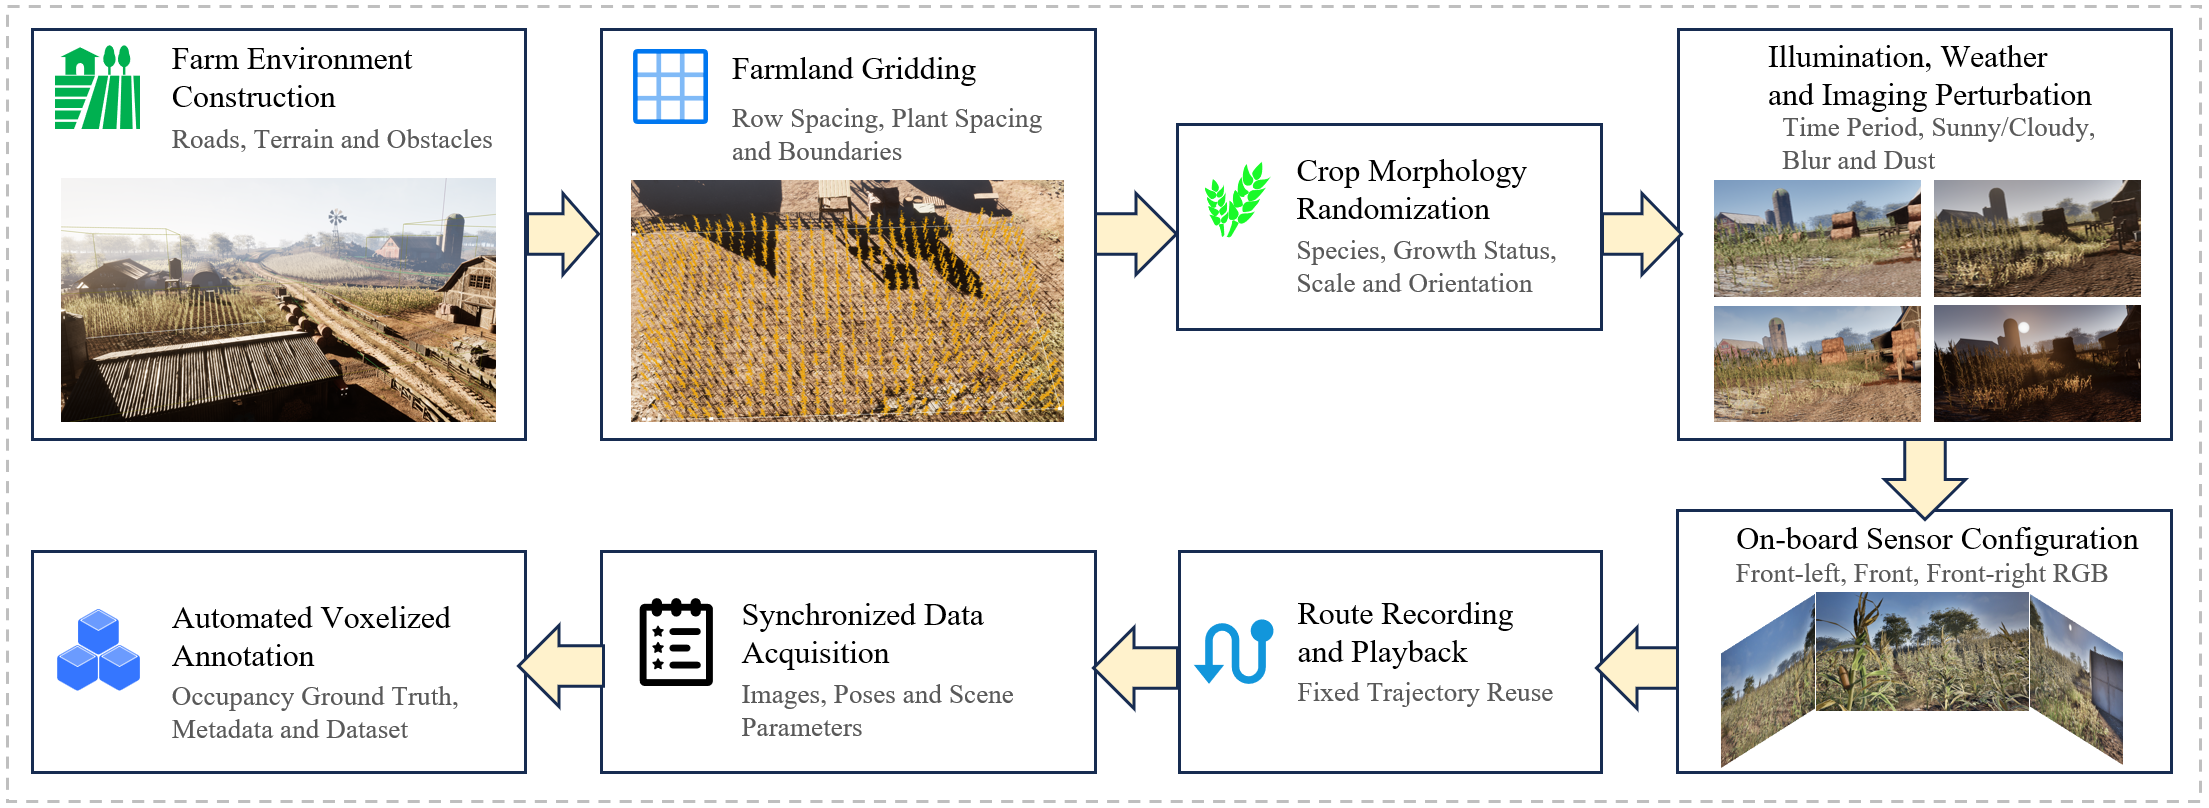
\includegraphics[width=1\linewidth]{synthetic.png}
\caption{Construction pipeline of the farmland simulation data-acquisition system.}
\label{fig:synthetic}\end{figure}

We first record multiple driving trajectories of the tractor in the simulated field and replay each route under different combinations of crop type, growth stage, illumination period, and weather, producing diverse combinations of field scenes and motion trajectories. To reduce appearance discrepancies between simulation and real acquisition, the system additionally applies imaging perturbations to RGB images with prescribed probabilities, including motion blur, lens stains, and airborne dust particles. Unlike real-world datasets such as nuScenes, the simulation engine directly exports camera poses, scene semantics, and voxel occupancy states, avoiding laborious per-frame point-cloud semantic labeling, multi-frame spatiotemporal registration, and voxel-label generation. For each frame, the forward space in the vehicle-local coordinate frame is divided into a regular 3D voxel grid, and dense occupancy ground truth is automatically generated from scene geometry and semantic labels. Raw environmental semantics are merged into six task-specific classes: free space, crop, soil ground, drivable area, other vegetation, and other obstacles. Each sample thus contains RGB images from three views, corresponding 3D semantic occupancy labels, and pose and scene-parameter metadata, forming a multimodal agricultural dataset for training and evaluating visual occupancy prediction.

\subsubsection{AgriOcc-Dataset}\label{sec:agriocc_dataset}
Following this process, we construct AgriOcc-Dataset, a multi-view 3D semantic occupancy dataset for field agricultural robots. Each sequence contains synchronized RGB images from forward, forward-left, and forward-right views, camera intrinsics and extrinsics, robot poses, semantic occupancy labels, and valid-voxel masks. At loading time, labels are mapped to the six classes \texttt{free}, \texttt{crop}, \texttt{soil\_ground}, \texttt{drivable}, \texttt{other\_vegetation}, and \texttt{other\_obstacle}; forward voxel supervision is generated in the robot coordinate frame.

The dataset contains 298 simulated driving sequences recorded at 10\,Hz, totaling approximately 194k frames. To avoid excessive repetition of similar scenes, we downsample to 2\,Hz, obtaining 38.8k samples. Among them, 248 sequences (32,385 frames) are used for training and 50 sequences (6,477 frames) for validation. The data cover ten crops: cabbage, carrot, corn, cucumber, potato, radish, red beet, sunflower, tomato, and wheat. Each crop includes early, mid, and mature growth stages; dawn, morning, noon, evening, and night; and cloudy and sunny weather. Figure~\ref{fig:crop_distribution} shows the crop composition.
\begin{figure}[pos=htbp]\centering
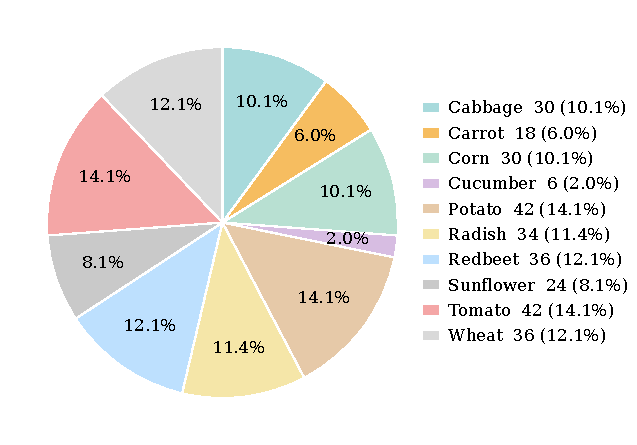
\includegraphics[width=0.5\linewidth]{crop_distribution.pdf}
\caption{Crop composition of AgriOcc-Dataset. Sector area indicates the proportion of each crop.}
\label{fig:crop_distribution}\end{figure}
\begin{figure}[pos=htbp]\centering
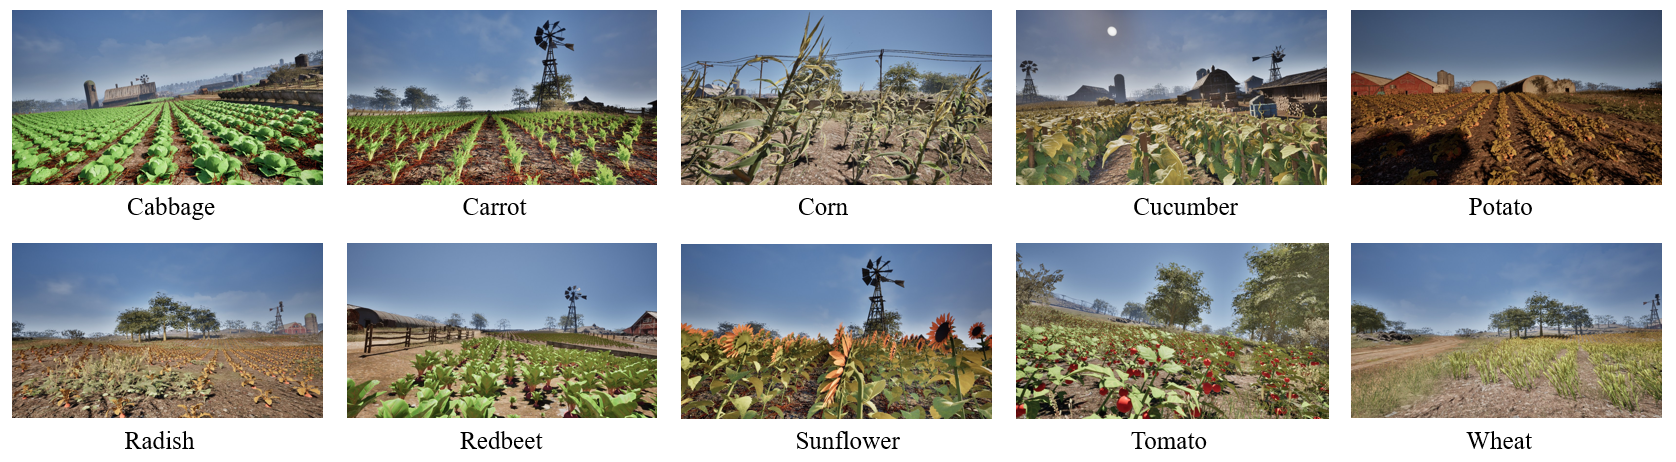
\includegraphics[width=\linewidth]{dataset.png}
\caption{Scene examples of the ten crops in AgriOcc-Dataset.}
\label{fig:dataset}\end{figure}

\subsection{Overall AgriOcc architecture}\label{sec:architecture}
Figure~\ref{fig:overview} presents the overall AgriOcc architecture. The image encoder uses ResNet-101 and FPN to extract four-level 2D features. A six-layer GeoVis-BEV encoder then uses GVAD as the context-enhancement unit for BEV tokens: within each layer, GVAD first combines local deformable updates with visibility-guided global anchors to supplement reliable spatial context for current BEV queries; spatial cross-attention subsequently aggregates geometrically aligned visual evidence from multi-scale images. After layer-wise updates, the encoder outputs $100\times100$ BEV tokens with 256 channels. A three-layer occupancy decoder provides multi-level supervision. In its final layer, Agri-AMoE lifts BEV tokens into a 3D feature volume and predicts six-class logits at 25 height positions. Thus, AgriOcc uses GVAD to optimize visibility-driven global-context modeling during BEV encoding, uses the NearFar layout to focus early encoding computation on fine near-field structures, and uses Agri-AMoE to adaptively model local 3D structures.
\begin{figure}[pos=htbp]\centering

\includegraphics[width=\linewidth]{overview.png}
\caption{Overall AgriOcc architecture. Three forward-facing images are processed by ResNet--FPN to produce four-scale features. The six-layer GeoVis-BEV encoder executes GVAD, image spatial cross-attention, and feed-forward updates in sequence in each layer. NearFar applies its near--far query layout in the first five layers and restores dense BEV before the sixth layer. The three-layer occupancy decoder provides multi-level supervision; its final layer uses Agri-AMoE to lift BEV tokens into a 3D feature volume and outputs $100\times100\times25\times6$ semantic logits.}
\label{fig:overview}\end{figure}

\subsection{GeoVis-BEV encoder}\label{sec:bev-encoder}
Semantic occupancy prediction must reconstruct dense 3D semantic space in the robot coordinate frame from limited-view 2D visual evidence. In farmland, crop-canopy occlusion, regular repetitive row-and-ridge textures, and the limited field of view of forward-facing cameras leave many BEV cells without direct or reliable observations. The resulting projection holes and semantic ambiguity can oversmooth crop--free-space boundaries or cause weakly observed regions to inherit erroneous local evidence. Meanwhile, details of near-field crops, furrows, and obstacles directly determine traversable space, whereas far-field observations are sparser. A uniform query density and context aggregation over the entire BEV plane neither selectively compensates weakly visible regions nor allocates sufficient computation to fine near-field modeling.

Built on BEVFormer's multi-camera BEV encoding framework\citep{li2022bevformer}, we propose the GeoVis-BEV encoder. It constructs local evidence through geometric projection, selects reliable context through visibility, and configures encoding budget by task distance. Across layer-wise image-conditioned updates, the encoder jointly models geometric relations, observation visibility, and near--far query density, transforming limited multi-camera observations into BEV representations with both local boundaries and globally consistent structure. For the BEV tokens input to layer $l$, the encoder sequentially strengthens local structures and reliable long-range context with GVAD, aggregates geometrically aligned multi-scale image features through spatial cross-attention, and updates representations with a feed-forward network. This process is repeated six times, yielding dense $100\times100$ BEV tokens with 256 channels.
\begin{figure}[pos=htbp]\centering
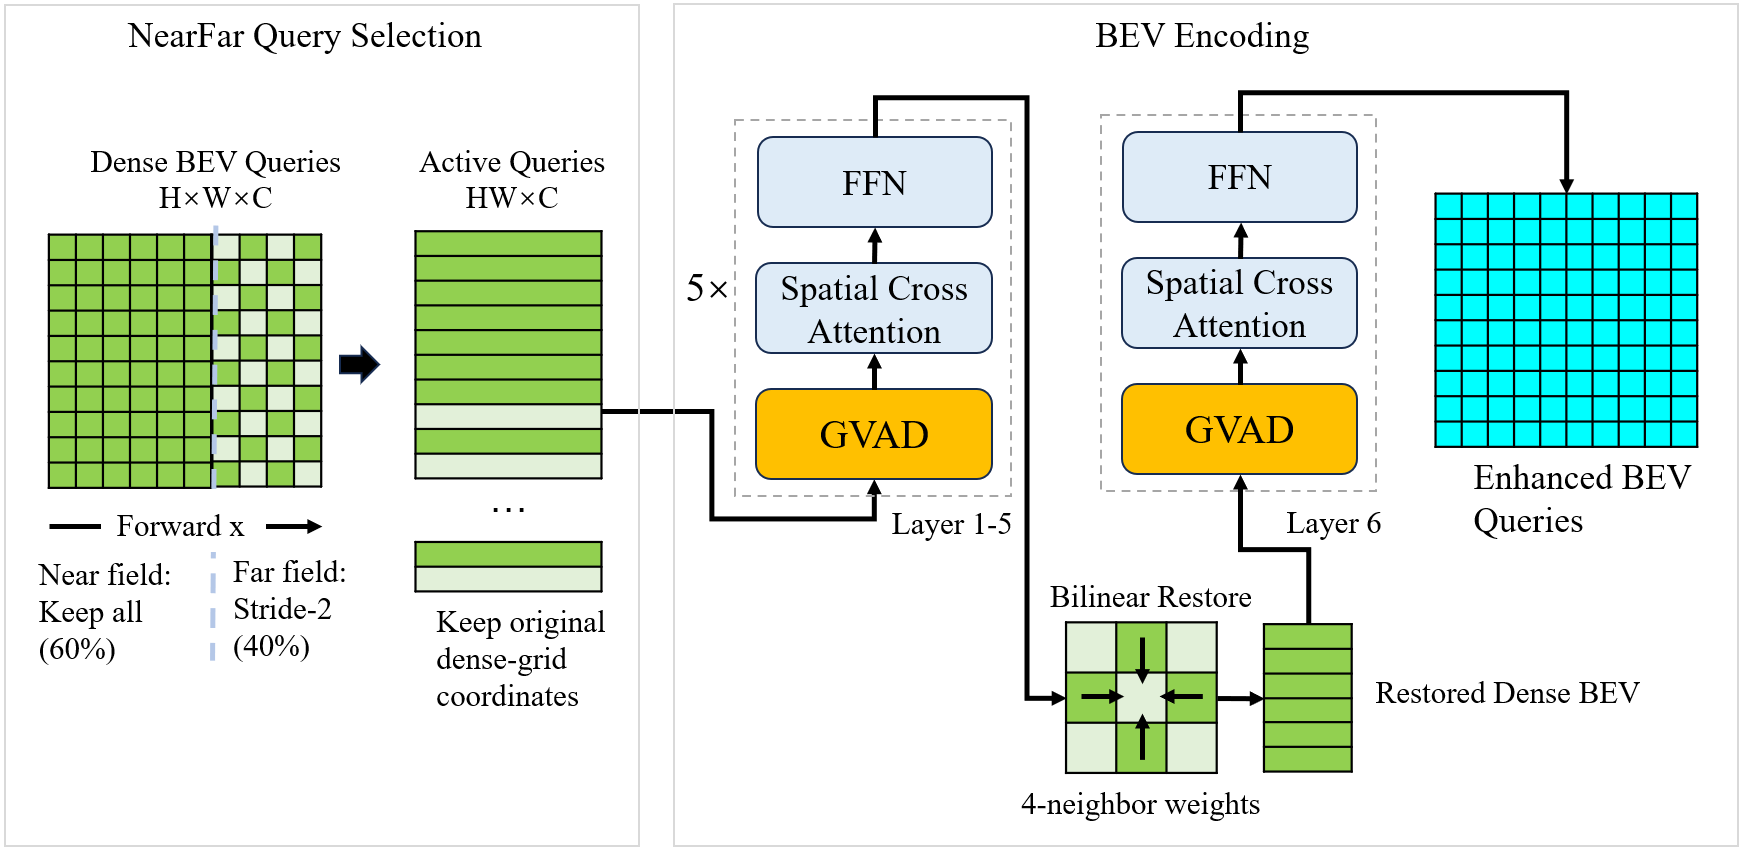
\includegraphics[width=\linewidth]{geovis-bev.png}
\caption{Overall architecture of the GeoVis-BEV encoder. Three forward-facing images are processed by ResNet--FPN and fed to a six-layer encoder. GVAD updates BEV tokens in every layer. NearFar retains dense near-field queries and regularly sparsely samples far-field queries in the first five layers; after restoration to a dense grid, the final layer performs image-conditioned refinement.}
\label{fig:geovis-bev-encoder}\end{figure}

\subsubsection{Geometry-Visible Anchor Deformable Attention}\label{sec:gvad}
GVAD is placed at the beginning of every GeoVis-BEV encoding layer, before image spatial cross-attention, to enhance BEV queries. It retains local projection detail while reading reliable long-range context according to cell visibility. Its inputs are the BEV tokens at layer $l$, $\bm{Q}^{l}=[\bm{q}_1,\ldots,\bm{q}_{N}]\in\R^{B\times N\times d}$, their positional encodings $\bm{E}^{l}=[\bm{e}_1,\ldots,\bm{e}_{N}]$, and the validity mask $\bm{M}\in\{0,1\}^{C_{\mathrm{cam}}\times B\times N\times Z}$ obtained by calibrated camera projection. Here, $B$, $N=HW$, and $d$ denote batch size, number of BEV tokens, and channel dimension; $H\times W$ is the BEV grid size; $C_{\mathrm{cam}}$ is the number of cameras; and $Z$ is the number of height reference points projected for each BEV column. $M_{c,b,i,z}=1$ indicates that reference point $z$ of BEV column $i$ in sample $b$ projects into camera $c$. Multi-camera, multi-height projection validity is reduced to token-level visibility:
\begin{equation}
m_{b,i}=\frac{1}{C_{\mathrm{cam}}Z}\sum_{c=1}^{C_{\mathrm{cam}}}\sum_{z=1}^{Z}M_{c,b,i,z}\in[0,1].
\end{equation}
We omit the batch index $b$ below. GVAD first applies layer normalization to positional-encoding-augmented inputs, $\tilde{\bm{q}}_i=\operatorname{LN}(\bm{q}_i+\bm{e}_i)$, then computes a local deformable branch and a geometry-visible anchor branch in parallel, and finally fuses them with visibility-gated residual connections. The local branch inherits BEVFormer's query-adaptive attention backbone\citep{li2022bevformer}; the anchor path combines sparse aggregation from Deformable DETR\citep{zhu2021deformable} with geometric querying from DETR3D\citep{wang2022detr3d} to explicitly assess observation reliability.

\paragraph{Local deformable branch.} This branch is deformable self-attention over BEV tokens. Given $(\bm{Q}^{l},\bm{E}^{l})$, it predicts a small set of sampling offsets and attention weights for each query and performs multi-head deformable aggregation in a local neighborhood of the BEV feature map, yielding a local update $\bm{d}_i$. Denoting this operation by $\mathcal{D}$,
\begin{equation}
\bm{d}_i=\mathcal{D}(\bm{q}_i,\bm{e}_i)-\bm{q}_i.
\end{equation}
It preserves structural continuity among neighboring tokens and provides more stable BEV queries for the following image spatial cross-attention.

\paragraph{Geometry-visible anchor branch.} To compensate for weakly visible queries using reliable regions, we uniformly divide the BEV plane into $H_a\times W_a$ tiles. We use $H_a=4$ and $W_a=8$, giving $K=H_aW_a=32$ anchors. For token $i$ in tile $a$, the anchor weight is determined jointly by content confidence and visibility:
\begin{equation}
s_{ia}=\bm{w}_c^\top\tilde{\bm{q}}_i+\gamma\log(m_i+\epsilon),\qquad
\alpha_{ia}=\softmax_{i\in a}(s_{ia}),\qquad
\bm{z}_a=\sum_{i\in a}\alpha_{ia}\tilde{\bm{q}}_i .
\end{equation}
Here, $\bm{w}_c$ is a learnable confidence projection, $\gamma$ is a learnable visibility scale, $\epsilon$ is a numerical-stability constant, $\alpha_{ia}$ is normalized within a tile, and $\bm{z}_a\in\R^d$ is the feature of visible anchor $a$. The same weights are applied to normalized 2D BEV-center coordinates $\bm{r}_i\in[0,1]^2$ to obtain $\bm{r}_a=\sum_{i\in a}\alpha_{ia}\bm{r}_i$. Each query then reads all anchors through multi-head attention with a distance bias:
\begin{equation}
A_{i,a}^{(h)}=\frac{(W_q^{(h)}\tilde{\bm{q}}_i)^\top(W_k^{(h)}\bm{z}_a)}{\sqrt{d_h}}-\rho_h\|\bm{r}_i-\bm{r}_a\|_2^2,\qquad
\pi_{i,a}^{(h)}=\softmax_a\left(A_{i,a}^{(h)}\right),
\end{equation}
\begin{equation}
\bm{g}_i=W_o\operatorname{Concat}_{h=1}^{H_{\mathrm{head}}}
\left(\sum_{a=1}^{K}\pi_{i,a}^{(h)}W_v^{(h)}\bm{z}_a\right).
\end{equation}
Here $h$ indexes attention heads, $H_{\mathrm{head}}$ is the number of heads, and $d_h=d/H_{\mathrm{head}}$; $W_q^{(h)}$, $W_k^{(h)}$, $W_v^{(h)}$, and $W_o$ are learnable linear projections. $\rho_h=\operatorname{softplus}(\delta_h)\geq0$ is the learnable distance-decay coefficient for head $h$, with unconstrained parameter $\delta_h$. The path can thus read globally while preferentially aggregating geometrically closer reliable anchors.

\paragraph{Visibility-gated fusion.} The outputs of the two branches and the original query are fused residually. Specifically, the gate $\eta_i$ is predicted from normalized features and token visibility and decreases as visibility increases:
\begin{equation}
\eta_i=\sigma\left(f_g([\tilde{\bm{q}}_i,m_i])\right)(1-\beta m_i),\qquad
\bm{q}_i'=\bm{q}_i+\bm{d}_i+\eta_i\bm{g}_i,
\end{equation}
where $f_g$ is a learnable gate projection, $[\cdot,\cdot]$ denotes channel concatenation, $\sigma$ is the Sigmoid function, $\beta=0.75$ is a fixed visibility-decay coefficient, and $\bm{q}_i'$ is the GVAD output token. Weakly visible cells therefore receive stronger anchor-context correction, whereas directly visible regions rely primarily on the local branch to prevent global information from overwriting fine boundaries. Figure~\ref{fig:gvad} illustrates the dual-path architecture.
\begin{figure}[pos=htbp]\centering
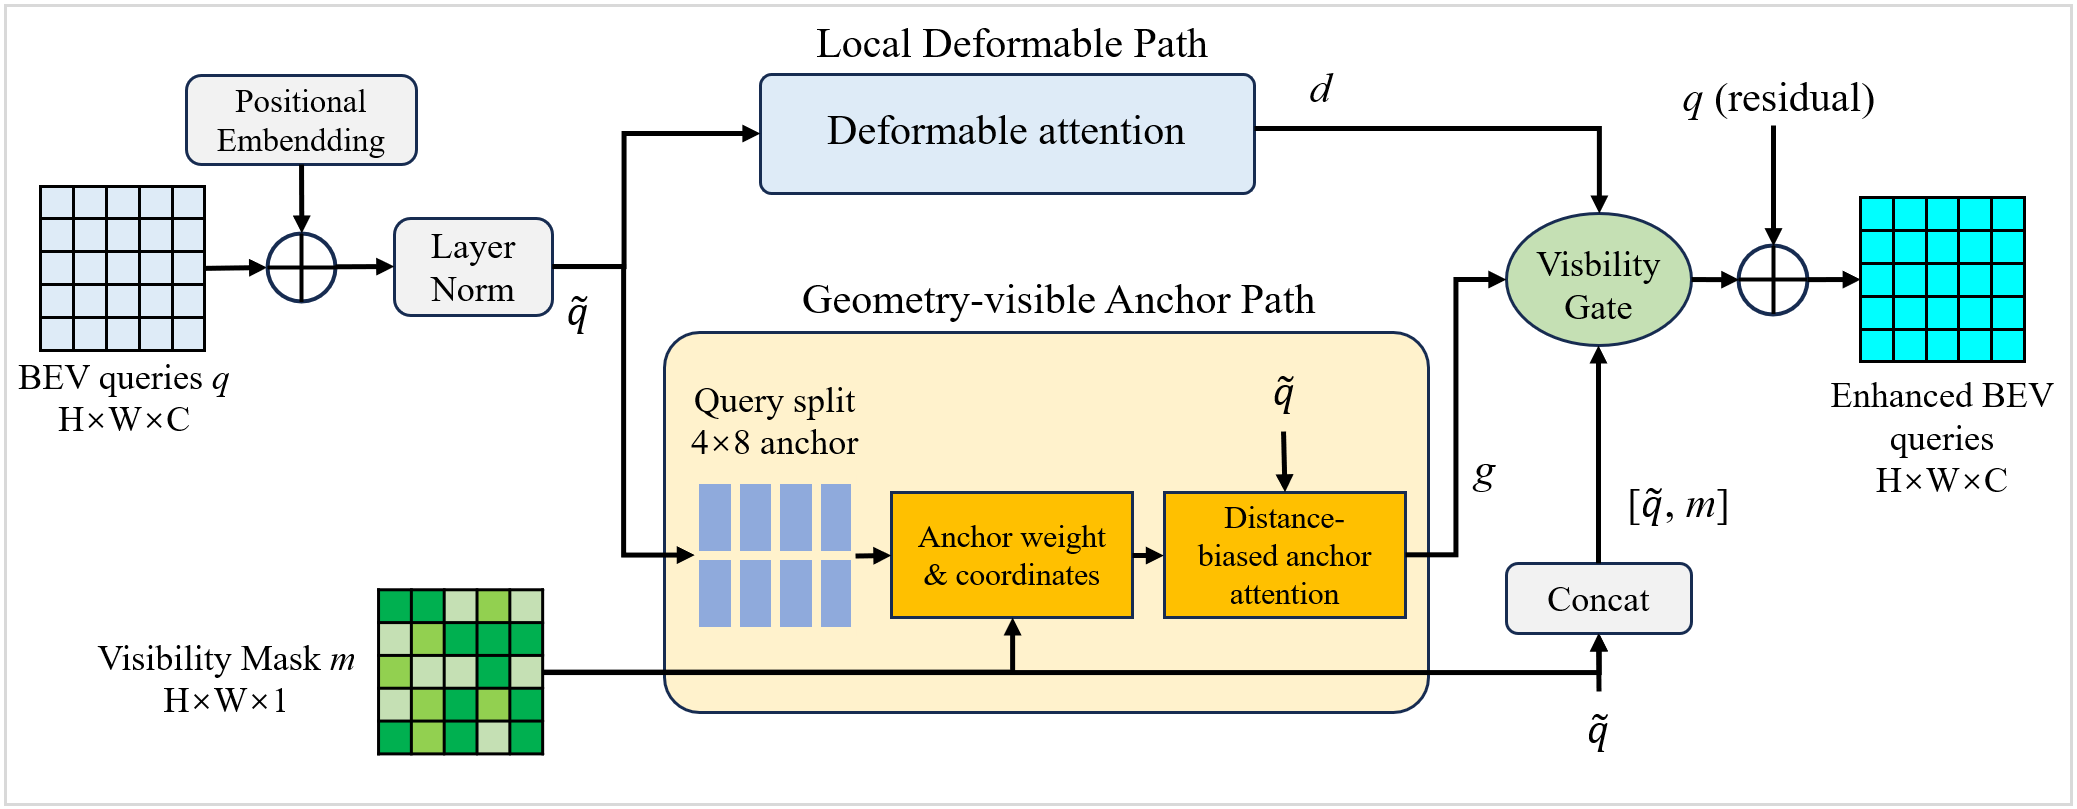
\includegraphics[width=\linewidth]{gvad.png}
\caption{GVAD architecture. The camera-projection mask is first reduced to visibility for each BEV token. The local deformable branch predicts sampling locations and weights from queries to form local BEV updates. The geometry-visible anchor branch divides the BEV plane into $4\times8$ tiles, constructs 32 anchors weighted by feature confidence and visibility, and forms anchor context through distance-biased multi-head attention. The two branches are fused through visibility gating and residual connections into enhanced BEV tokens.}
\label{fig:gvad}\end{figure}

\subsubsection{NearFar BEV query layout}\label{sec:nearfar}
The NearFar query layout prioritizes early encoding computation for the near field, which is more critical to planning and obstacle avoidance and has richer image evidence, while retaining a dense final occupancy grid. Along the forward-distance axis of the BEV grid ($0$--$20\,$m ahead), the first $60\%$ of cells (within 12\,m) are defined as the near field and retain all queries. In the remaining $40\%$ far-field cells, one query is retained every two cells, producing regular 2D sparse sampling. The first five encoding layers process the active-token set comprising dense near-field and sparse far-field queries. At inactive far-field locations, features are restored using bilinear weights from four neighboring active tokens. The final layer restores the complete $100\times100$ grid and performs dense, image-conditioned cross-attention. This arrangement avoids completing far-field semantics through query interpolation alone and leaves existing occupancy decoder heads unchanged. In sparse layers, GVAD still bins tokens according to their original dense BEV coordinates, so anchor coverage is unaffected by sparse sampling.

As shown in Fig.~\ref{fig:geovis-bev-encoder}, the NearFar layout retains the complete near-field grid to express fine geometry of crops, furrows, and obstacles, sparsely samples the far field regularly, and restores the full feature map before final dense image cross-attention.

\subsection{Agricultural Structure-Adaptive Mixture-of-Experts 3D occupancy decoder}\label{sec:agri-amoe}
Farmland occupancy space is markedly anisotropic: crop rows and furrows exhibit long-range continuity and periodic alternation on the ground plane, whereas crop canopies, soil, and obstacles have distinct boundary shapes along height. Inter-plant gaps and crop--free-space boundaries often occupy only a small number of voxels. If 2D BEV tokens are mapped independently and directly to classes at each height, the decoder cannot coordinate planar detail and vertical structure at neighboring positions, resulting in oversmoothing in fine-grained regions. The final occupancy head must thus restore the height dimension and adaptively select suitable receptive fields and directional modeling according to local 3D structural complexity.

Inspired by the use of mixture-of-experts occupancy decoding in \citep{shi2026oneocc}, we design the Agricultural Structure-Adaptive Mixture-of-Experts 3D occupancy decoder (Agri-AMoE). Rather than defining experts for generic urban scenes, we define expert forms from anisotropic farmland structures along planar, vertical, and contextual directions, and use interpretable gradient energy as the routing signal, linking expert specialization directly to agricultural structures such as crop rows, furrows, and canopies. For final-layer BEV features $\bm{Q}\in\R^{B\times HW\times C}$, a linear mapping and reshape first produce a 3D volume feature with $C_a$ channels:
\begin{equation}
\bm{F}_0=\operatorname{reshape}(W_{\mathrm{lift}}\bm{Q})\in\R^{B\times C_a\times Z\times H\times W}.
\end{equation}
Here $C$ is the input BEV-token channel count, $H$ and $W$ are planar BEV-grid dimensions, $Z$ is the number of height bins, $W_{\mathrm{lift}}$ is a learnable lifting mapping, and $\operatorname{reshape}(\cdot)$ only rearranges mapped tokens into the volume. We use $C_a=96$ and $Z=25$. Global 3D pooling and an MLP generate channel-attention weights to enhance the volume:
\begin{equation}
\bm{F}=\bm{F}_0\odot\sigma\!\left(f_c(\operatorname{GAP}(\bm{F}_0))\right).
\end{equation}
$\operatorname{GAP}$ is global average pooling over $Z$, $H$, and $W$; $f_c$ is a learnable channel mapping; $\sigma$ is the Sigmoid function; and $\odot$ is elementwise multiplication. The enhanced $\bm{F}$ is passed in parallel to three anisotropic experts and a routing branch. $\mathcal{E}_1$ uses $1\times3\times3$ depthwise separable convolutions to encode inter-plant planar detail, $\mathcal{E}_2$ uses $3\times1\times1$ convolutions for vertical structures, and $\mathcal{E}_3$ uses $1\times3\times3$ convolutions with dilation 2 for larger planar context.

The router assigns expert weights to every voxel according to spatial saliency and local structural variation of $\bm{F}$. Spatial saliency is computed from channel-wise mean and maximum values through a $3\times3\times3$ convolutional spatial mapping $f_s$:
\begin{equation}
\bm{S}=\sigma\!\left(f_s([\operatorname{mean}_c(\bm{F}),\operatorname{max}_c(\bm{F})])\right).
\end{equation}
Here $\operatorname{mean}_c$ and $\operatorname{max}_c$ are channel-wise average and maximum aggregation, and $\bm{S}$ is a per-voxel spatial-saliency map. To align expert selection with 3D structural complexity, the router also calculates finite-difference energy in three spatial directions:
\begin{equation}
\bm{E}=\operatorname{mean}_c\!\left((\nabla_x\bm{F})^2+(\nabla_y\bm{F})^2+(\nabla_z\bm{F})^2\right).
\end{equation}
$\nabla_x$, $\nabla_y$, and $\nabla_z$ are gradients along the three spatial axes; $\bm{E}$ thus measures local structural variation per voxel. Using $[\log(1+\bm{E}),\bm{S}]$ as input, the router outputs three normalized expert weights at temperature $\tau=1$:
\begin{equation}
\bm{\alpha}=\operatorname{Softmax}\!\left(g([\log(1+\bm{E}),\bm{S}]) / \tau\right),
\end{equation}
where $g$ is a three-route mapping composed of two $1\times1\times1$ convolution layers, group normalization, and ReLU, and $\alpha_k$ is expert $k$'s weight at each voxel. Finally, routing weights fuse the already computed expert outputs:
\begin{equation}
\bm{F}'=\operatorname{ReLU}\!\left(\bm{F}+\operatorname{GN}\!\left(\sum_{k=1}^{3}\alpha_k\mathcal{E}_k(\bm{F})\right)\right),\qquad
\bm{O}=W_o\bm{F}',
\end{equation}
where $\operatorname{GN}$ denotes group normalization, $\operatorname{ReLU}$ is the nonlinear activation, $W_o$ is a $1\times1\times1$ classification convolution, and $\bm{O}\in\R^{B\times6\times Z\times H\times W}$ contains final semantic logits. Figure~\ref{fig:agri-amoe} illustrates the module.
\begin{figure}[pos=htbp]\centering

\includegraphics[width=\linewidth]{agri-amoe.png}
\caption{Agri-AMoE 3D occupancy decoder. 2D BEV tokens are lifted into a 3D volume and enhanced by channel attention. Enhanced features are passed in parallel to three anisotropic experts and used to compute spatial saliency and three-direction gradient energy for per-voxel routing weights. The weighted expert outputs are summed, residually fused, and classified.}
\label{fig:agri-amoe}\end{figure}

\subsection{Overall optimization objective}\label{sec:loss}
The occupancy loss follows the multi-level voxel-supervision paradigm of SurroundOcc and OpenOccupancy\citep{wei2023surroundocc,wang2023openoccupancy}. It comprises class cross-entropy, semantic-scale loss, geometric-scale loss, and a Lov\'{a}sz-Softmax term; its detailed calculation is identical to those works and is therefore not repeated.

\section{Experiments}\label{sec:experiments}
\subsection{Datasets and evaluation protocol}\label{sec:data}
\paragraph{AgriOcc-Dataset} Most experiments are conducted on AgriOcc-Dataset (Section~\ref{sec:dataset_construction}). AgriOcc uses forward, forward-left, and forward-right cameras to predict occupancy over a $20\,\mathrm{m}\times20\,\mathrm{m}$ area in front of the robot (lateral extent $\pm10\,$m).
\paragraph{ORAD-3D} To assess sim-to-real transfer, Section~\ref{sec:sim2real} evaluates AgriOcc on real off-road and farmland occupancy prediction using ORAD-3D\citep{chen2025orad3d}.
\paragraph{Metrics} We report mIoU and class-wise IoU. For class $c$, $\IoU_c=\mathrm{TP}_c/(\mathrm{TP}_c+\mathrm{FP}_c+\mathrm{FN}_c)$; mIoU is the arithmetic mean across valid classes.

\subsection{Implementation details}\label{sec:implementation}
AgriOcc uses an ImageNet-pretrained ResNet-101 image encoder, a six-layer GeoVis-BEV encoder, and a three-layer occupancy decoder. The input size is $512\times288$, and the voxel range is $[0,20]\times[-10,10]\times[-2,3]\,\mathrm{m}$ at $0.2\,\mathrm{m}$ resolution. We use AdamW with initial learning rate $2\times10^{-4}$, weight decay 0.01, a cosine schedule, and 500 linear warm-up iterations. The effective global batch size is 24; training lasts 8 epochs on four RTX 4090 GPUs.

\subsection{Comparison with existing methods}\label{sec:comparison}
Table~\ref{tab:main} compares occupancy prediction on AgriOcc-Dataset. SurroundOcc\citep{wei2023surroundocc}, SparseOcc\citep{tang2024sparseocc}, and COTR\citep{ma2024cotr} are current-frame semantic-occupancy methods; Drive-OccWorld\citep{yangDrivingOccupancyWorld2025} and IR-WM\citep{mei2025irwm} predict current and future occupancy. AgriOcc outperforms all compared methods, indicating that GeoVis-BEV and the agricultural structure-adaptive decoder transform image geometry into more consistent spatial occupancy. Gains are particularly evident for ground, drivable areas, and complex vegetation/obstacle classes, demonstrating robust joint modeling of large-scale field layout and local obstacle boundaries. Crop remains difficult because inter-plant separation and leaf occlusion cause semantic mixing during single-frame projection and voxelization.

SurroundOcc, SparseOcc, and COTR mainly target urban surround-view driving. Their uniform spatial queries and urban-road priors do not directly adapt to inter-row occlusion, elongated crops, and fine near-field boundaries in agricultural forward views. IR-WM and Drive-OccWorld, by contrast, exploit historical states, action conditions, and future rollouts for world modeling and planning. Since our protocol evaluates current-frame occupancy only, these additional capabilities cannot be fully converted into current-voxel accuracy, while multi-step joint optimization complicates representation learning. Their lower current-frame scores therefore reflect a mismatch of task objective and inductive bias, not a lack of ability to predict future states or support planning.
\begin{table}[pos=htbp]\centering
\caption{3D semantic occupancy results on the AgriOcc-Dataset validation set (\%). Parameter count is the number of trainable parameters. SurroundOcc, SparseOcc, and COTR are current-frame methods; Drive-OccWorld and IR-WM are world models also predicting future occupancy, for which only current-frame output is compared.}
\label{tab:main}\fontsize{9}{11}\selectfont\setlength{\tabcolsep}{2.6pt}
\begin{threeparttable}\begin{tabular}{lrrrrrrrr}\toprule
Method & Params. (M) & mIoU & Free & Crop & Soil & Drivable & Other veg. & Other obs. \\\midrule
SurroundOcc & 222.38 & 50.50 & 88.95 & 25.20 & 63.44 & 58.92 & 36.79 & 29.69 \\
SparseOcc & 58.14 & 37.10 & 83.53 & 17.66 & 38.99 & 34.02 & 25.82 & 22.31 \\
COTR & 37.17 & 36.50 & 91.11 & 8.59 & 54.48 & 30.88 & 26.50 & 7.42 \\
Drive-OccWorld & 60.68 & 35.15 & 85.52 & 19.63 & 40.29 & 29.64 & 21.06 & 14.77 \\
IR-WM & 60.68 & 35.15 & 85.52 & 19.63 & 40.29 & 29.66 & 21.06 & 14.76 \\\midrule
\textbf{AgriOcc} & \textbf{55.74} & \textbf{56.99} & \textbf{91.11} & \textbf{28.82} & \textbf{74.03} & \textbf{68.27} & \textbf{43.57} & \textbf{36.15} \\\bottomrule
\end{tabular}\end{threeparttable}\end{table}
Figure~\ref{fig:qualitative_comparison} presents qualitative comparisons for three representative farmland scenes. AgriOcc preserves better spatial continuity in crop rows, ground boundaries, and semantic layouts across near and far regions, and more reliably retains local obstacle structures.
\begin{figure}[pos=htbp]\centering
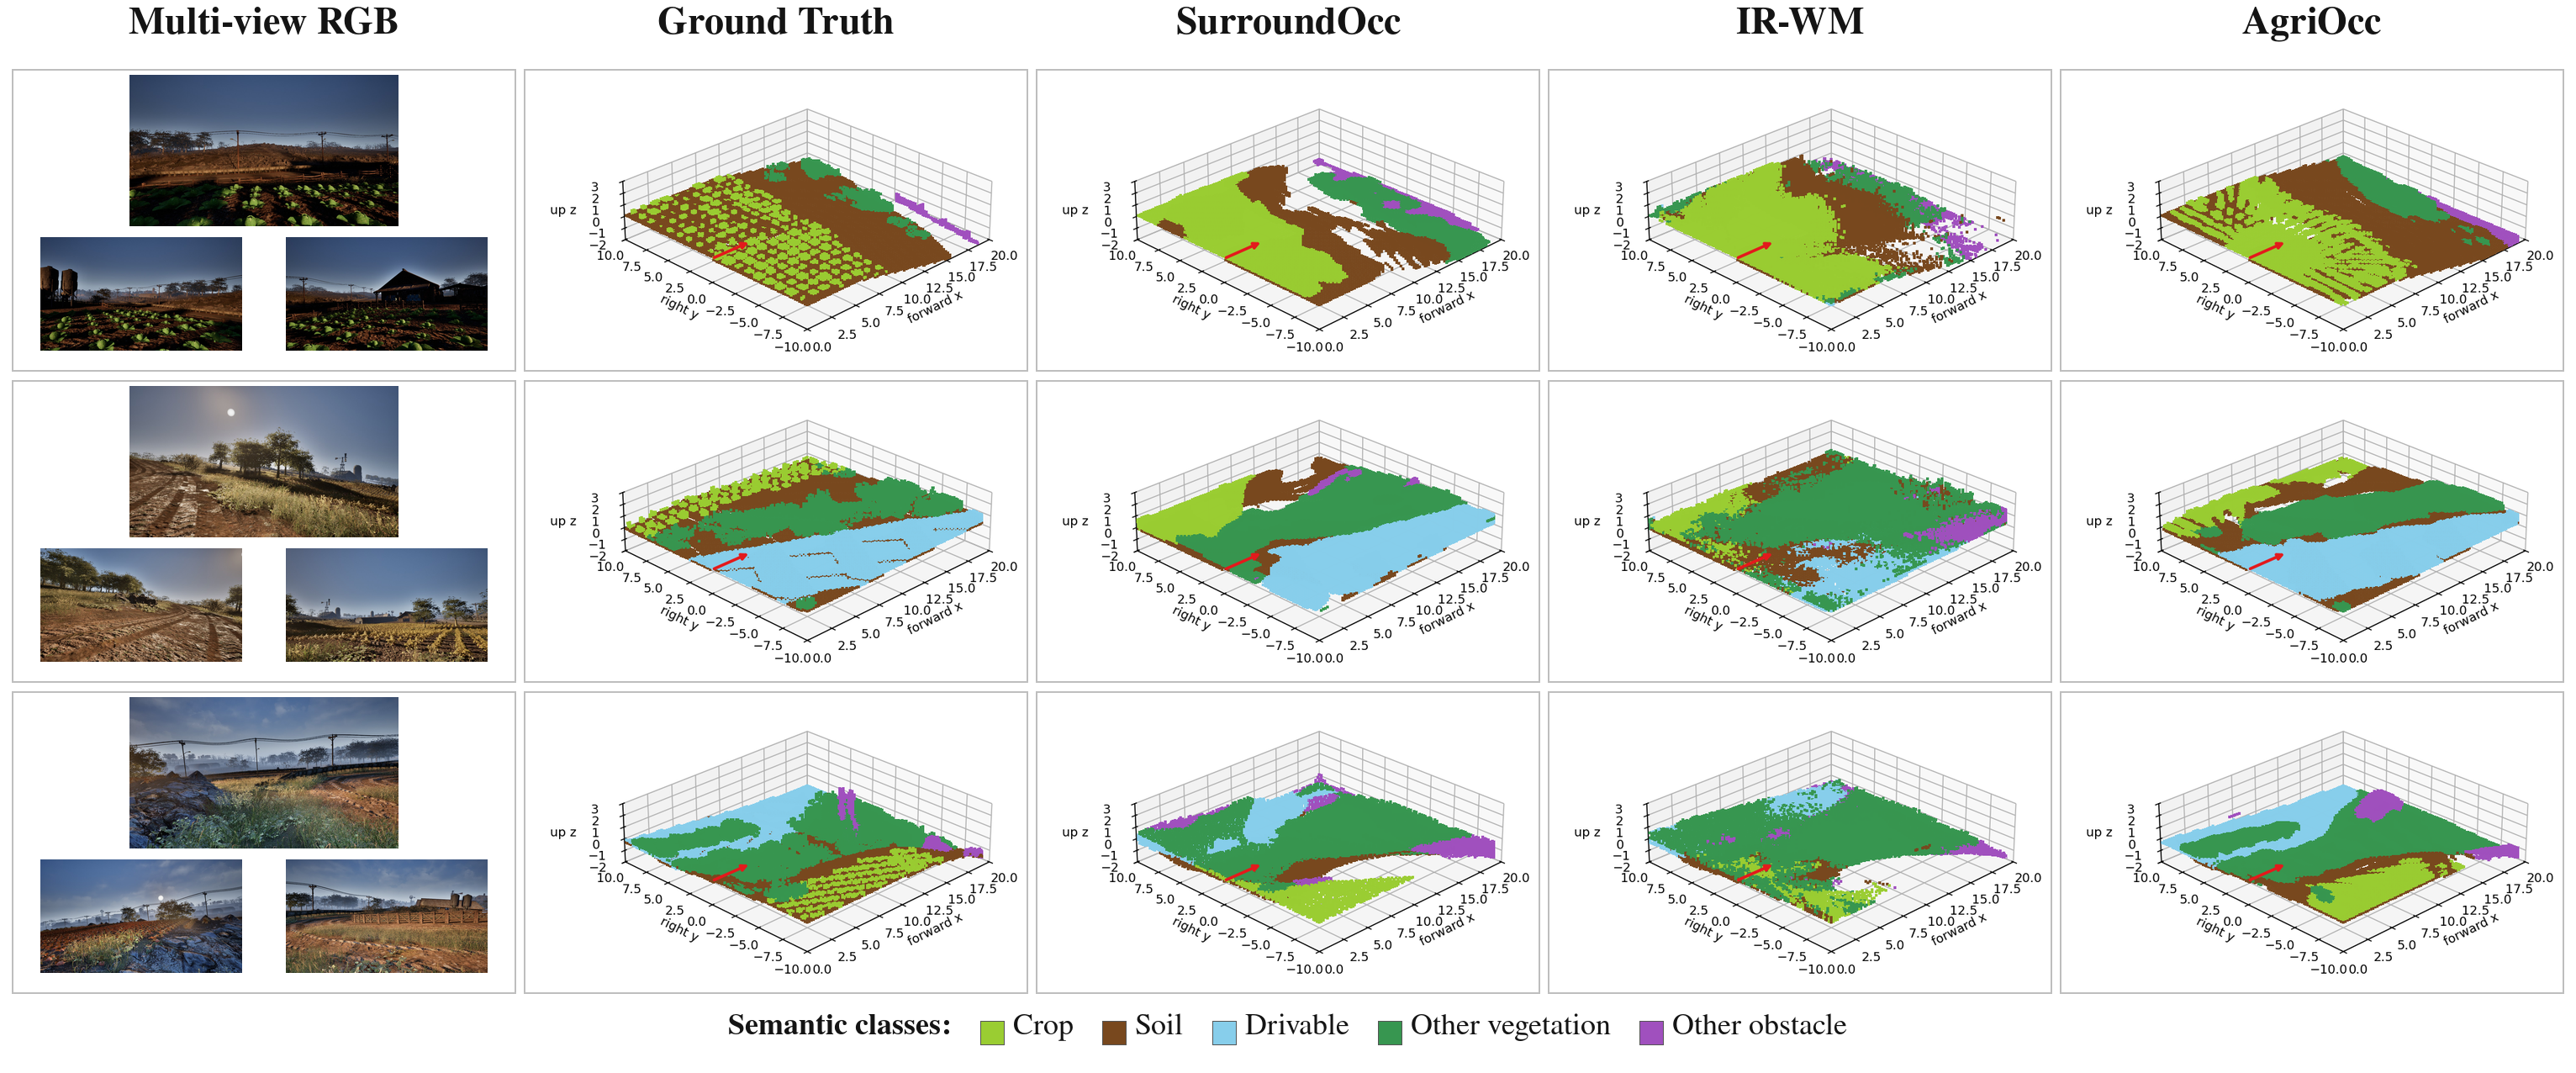
\includegraphics[width=\linewidth]{qualitative_comparison_3x5.png}
\caption{Qualitative comparison on AgriOcc-Dataset. Each row is a sample with different crops, illumination, and scene conditions. From left to right: three input RGB images, ground truth, and current-frame 3D semantic occupancy predictions from SurroundOcc, IR-WM, and AgriOcc. Red arrows indicate driving direction.}
\label{fig:qualitative_comparison}\end{figure}

\subsection{Ablation study}\label{sec:ablation}
Table~\ref{tab:ablation} evaluates cumulative modules under the same data split and training budget. GVAD yields the largest gain (53.89\% to 56.24\%), indicating that visible anchors mitigate geometric ambiguity induced by occlusion and viewpoint change. Adding NearFar reaches 56.49\% mIoU (+0.25), but provides clear memory and throughput gains, showing that the task benefits from a spatial sampling layout matched to the robot's operational range and that the module's primary value is computational allocation rather than accuracy alone. Agri-AMoE finally achieves 56.99\%, complementing geometry encoding and near--far queries through adaptive 3D local/contextual representation.

With per-GPU batch size 2, NearFar reduces peak memory from 15.14\,GB to 10.68\,GB (a 29.5\% reduction relative to the +GVAD configuration) and training time by 13.1\%. As parameter counts are almost identical (55.08M versus 55.12M), this benefit is mainly due to fewer queries and enables larger micro-batches under the same memory budget.
\begin{table}[pos=htbp]\centering
\caption{Ablation study on AgriOcc-Dataset. A checkmark indicates an enabled module. Training time is estimated from mean iteration time and iteration count in epoch 8; all configurations use four RTX 4090 GPUs and effective global batch size 24. Memory is peak allocated memory per GPU, measured after warm-up at fixed per-GPU batch size 2.}
\label{tab:ablation}\fontsize{9}{11}\selectfont\setlength{\tabcolsep}{1.4pt}
\begin{tabular}{lccccccr}\toprule
Configuration & GVAD & NearFar & Agri-AMoE & Params. (M) & Memory (GB) & Training (min/epoch) & mIoU (\%) \\\midrule
Base & & & & 52.12 & 13.08 & 26.02 & 53.89 \\
+ GVAD & \checkmark & & & 55.08 & 15.14 & 42.93 & 56.24 \\
+ NearFar & \checkmark & \checkmark & & 55.12 & \textbf{10.68} & 37.28 & 56.49 \\
+ Agri-AMoE & \checkmark & \checkmark & \checkmark & \textbf{55.74} & 11.03 & 40.95 & \textbf{56.99} \\\bottomrule
\end{tabular}\end{table}

\subsection{Sim-to-real transfer to off-road scenes}\label{sec:sim2real}
We transfer an AgriOcc checkpoint trained on AgriOcc-Dataset to ORAD-3D\citep{chen2025orad3d}, evaluating its official test set and farmland subset. ORAD-3D uses a $100\times100\times16$ grid and nine classes, with class definitions following its official annotation protocol. Its surround-view configuration and class system differ from AgriOcc; we therefore use only the center forward camera's BEV embedding, replace the occupancy head for the target grid and class count, and train for alignment on ORAD-3D.

Table~\ref{tab:orad} compares AgriOcc-Dataset-pretrained target-domain adaptation, AgriOcc trained from scratch, and baselines reported by ORAD-3D. \texttt{Test} uses all classes, \texttt{Test\_farm} uses classes present in the farmland subset, and \texttt{Test (w/o Free)} follows the semantic-mIoU convention of ORAD-3D. OpenOcc, OccFormer, and SurroundOcc results are quoted from that paper\citep{chen2025orad3d}. With identical full target-domain data, two adaptation epochs after AgriOcc-Dataset pretraining achieve 11.17\% on \texttt{Test (w/o Free)}, higher than the from-scratch result (9.01\%) and the reported SurroundOcc result (7.60\%), while reducing target-domain training time from 54.1 to 18.5 minutes. Thus, simulated agricultural pretraining transfers image--BEV geometry and 3D semantic priors to real off-road scenes at lower adaptation cost.
\begin{table}[pos=htbp]\centering
\caption{Sim-to-real transfer results on ORAD-3D (\%). Both AgriOcc variants use the full ORAD-3D training set and only the center forward camera. The transfer model is initialized by AgriOcc-Dataset pretraining and adapted for two epochs. \texttt{Test (w/o Free)} excludes Free; \texttt{Test} is nine-class mIoU; \texttt{Test\_farm} is mIoU over classes in the farmland subset. Baseline results are from the ORAD-3D paper.}
\label{tab:orad}\fontsize{9}{11}\selectfont\setlength{\tabcolsep}{2.6pt}
\begin{tabular}{lrrrr}\toprule
Method & Training time (min) & Test (w/o Free) & Test & Test\_farm \\\midrule
OpenOcc\citep{jiang2024openocc} & -- & 5.83 & -- & -- \\
OccFormer\citep{zhang2023occformer} & -- & 7.45 & -- & -- \\
SurroundOcc\citep{wei2023surroundocc} & -- & 7.60 & -- & -- \\\midrule
AgriOcc (from scratch) & 54.1 & 9.01 & 18.16 & 31.83 \\\midrule
AgriOcc (pretrained transfer) & 18.5 & \textbf{11.17} & \textbf{20.11} & 39.45 \\\bottomrule
\end{tabular}\end{table}
\begin{figure}[pos=htbp]\centering
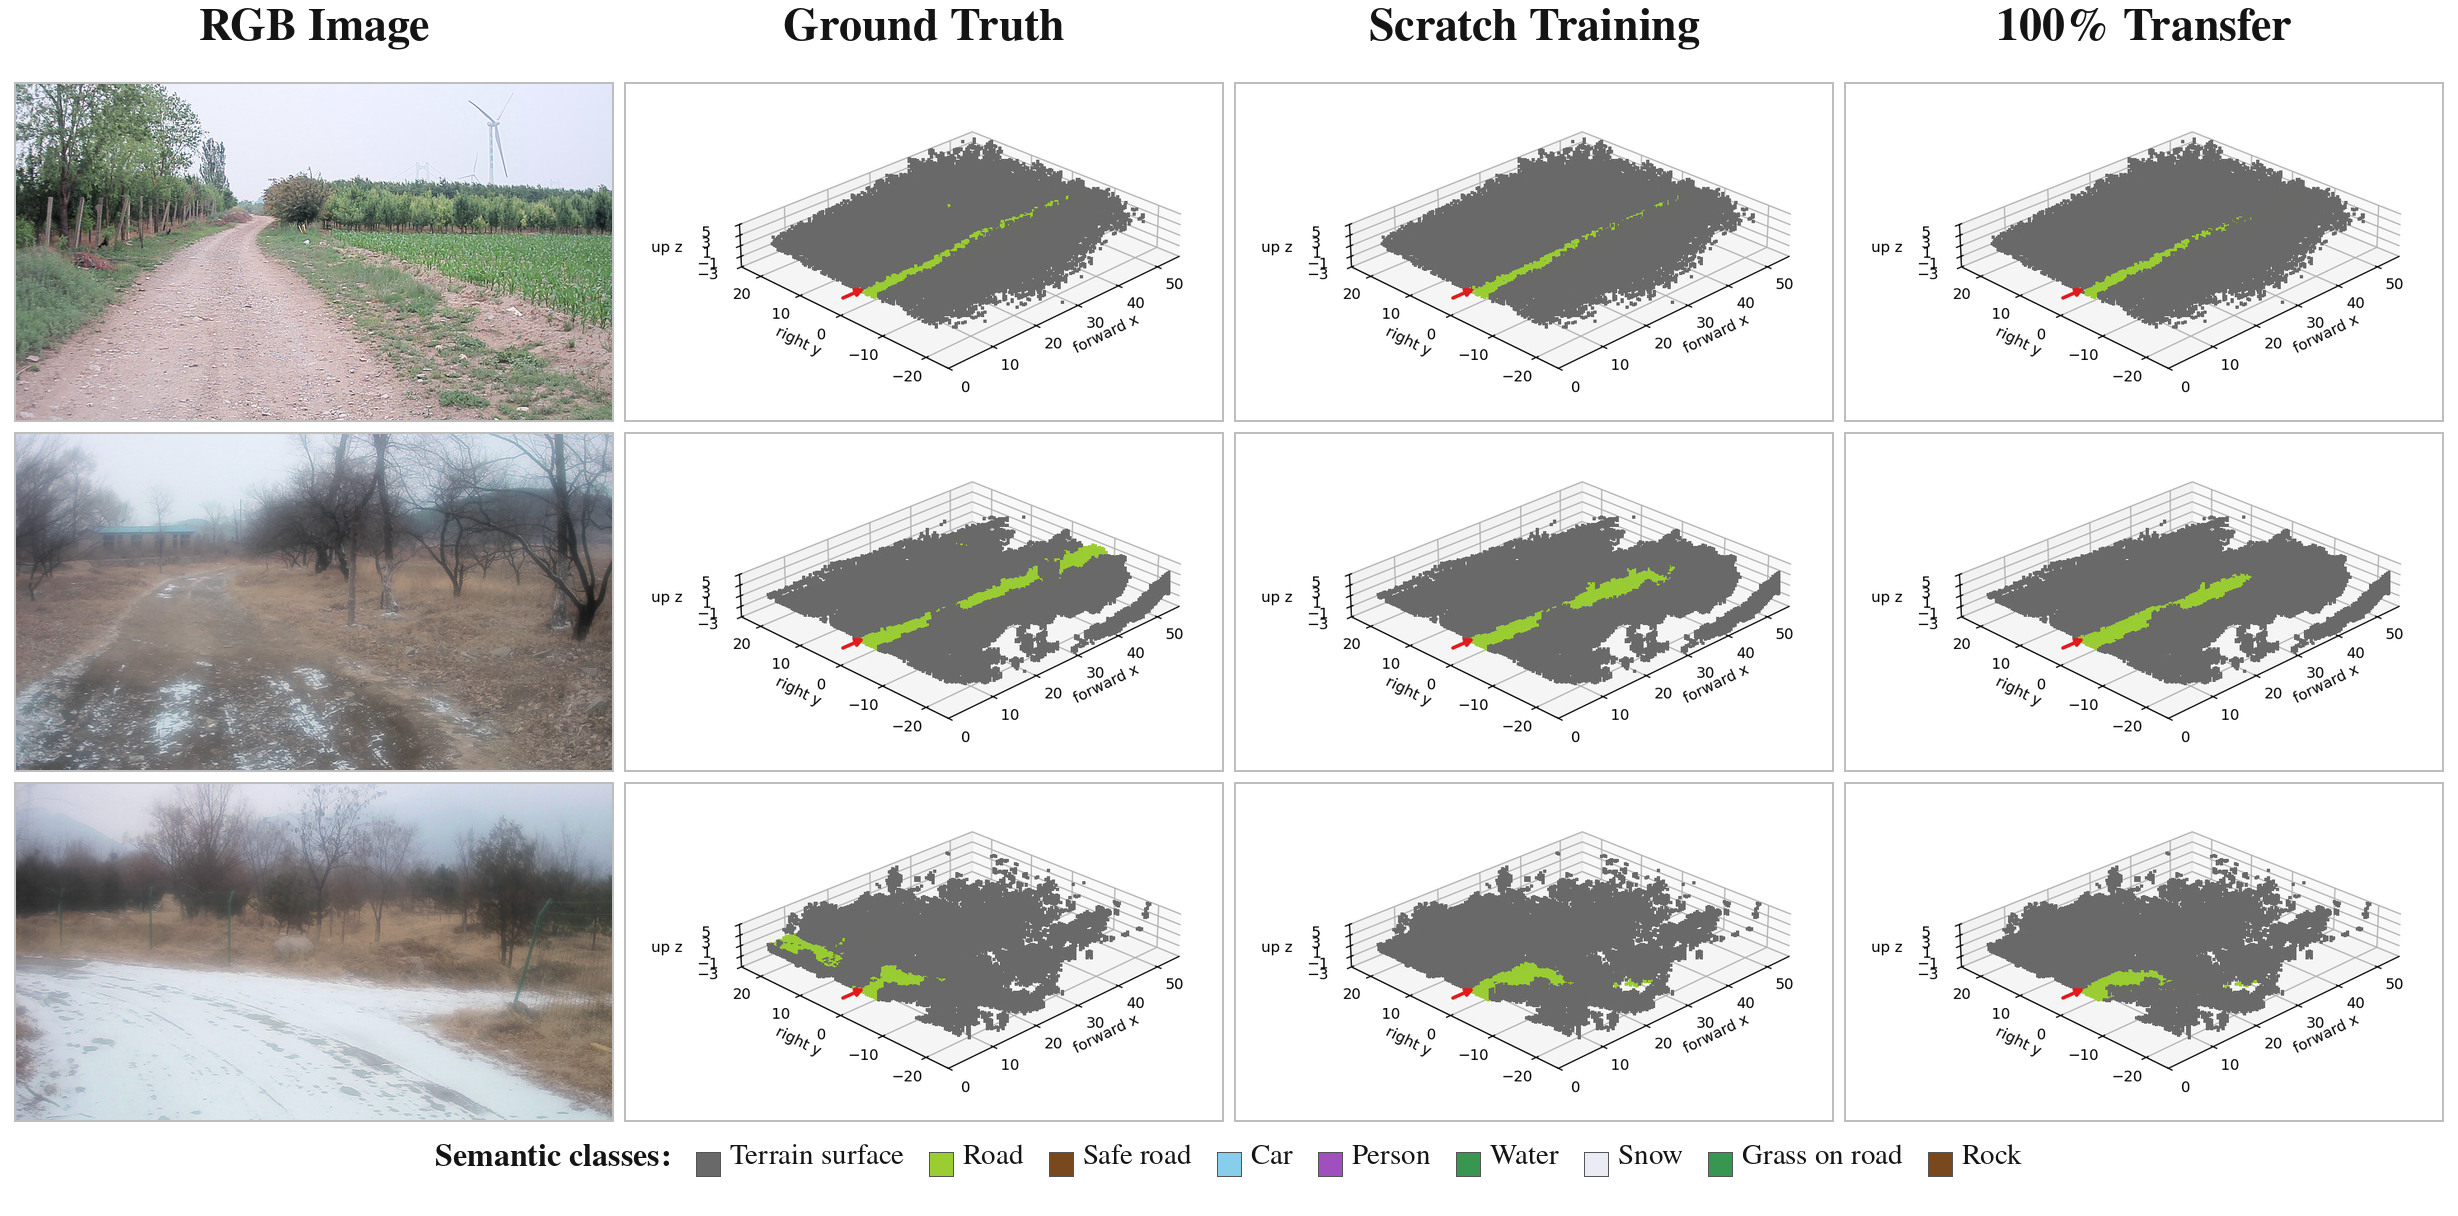
\includegraphics[width=\linewidth]{orad3d_transfer_qualitative.png}
\caption{Qualitative transfer comparison on ORAD-3D. Each row is the same official test sample. From left to right: input RGB image, ground truth, a model trained from scratch using all ORAD-3D training data, and a model transferred from AgriOcc-Dataset pretraining using all ORAD-3D training data (100\% Transfer).}
\label{fig:orad_qualitative}\end{figure}

\subsection{Voxel-resolution transfer}\label{sec:resolution_transfer}
AgriOcc-Dataset uses $0.2\,\mathrm{m}$ voxels, consistent with mainstream autonomous-driving semantic-occupancy benchmarks\citep{behley2019semantickitti,li2024sscbench}. However, $0.2\times0.2\times0.2\,\mathrm{m}$ voxels can quantize adjacent crops, narrow furrows, or local drivable boundaries into one grid cell during between-ridge navigation, inter-plant obstacle avoidance, and fine agricultural operations. Directly expanding the BEV encoder to $0.1\times0.1\times0.2\,\mathrm{m}$ increases the number of XY queries from $100\times100$ to $200\times200$, i.e., by a factor of four; consequently, the computational and memory costs of multi-scale image--BEV interaction, intermediate BEV activations, and 3D occupancy supervision increase substantially. We therefore collect a small $0.1\times0.1\times0.2\,\mathrm{m}$ simulation dataset with 19,300 samples, split equally into training and validation sets, to test whether learned standard-resolution 3D priors can be efficiently transferred to fine-resolution occupancy prediction.

The transfer model is first trained on the $0.2\times0.2\times0.2\,\mathrm{m}$ AgriOcc-Dataset. At $0.1\times0.1\times0.2\,\mathrm{m}$, \emph{query adaptation} freezes the backbone and learns only $200\times200$ high-resolution BEV queries. \emph{Refinement-head adaptation} retains and freezes the original $100\times100$ GeoVis-BEV encoder and Agri-AMoE decoder, training only a learned $2\times$ refinement head that fuses coarse occupancy logits and projected BEV features to output $200\times200\times25$ voxels. The control learns $200\times200$ high-resolution BEV and occupancy prediction from scratch on the same $0.1\,\mathrm{m}$ dataset without $0.2\,\mathrm{m}$ pretraining.
\begin{table}[pos=htbp]\centering
\caption{Transfer results at $0.1\,\mathrm{m}$ voxel resolution (IoU in \%; time is end-to-end wall-clock time for 8 epochs including per-epoch validation). Transfer methods first train at $0.2\times0.2\times0.2\,\mathrm{m}$, then freeze the backbone and adapt to $0.1\times0.1\times0.2\,\mathrm{m}$.}
\label{tab:resolution_transfer}\fontsize{9}{11}\selectfont\setlength{\tabcolsep}{2.4pt}\resizebox{\linewidth}{!}{%
\begin{tabular}{lrrrrrrrr}\toprule
Method & Time & mIoU & Free & Crop & Soil & Drivable & Other veg. & Other obs. \\\midrule
0.1 m from scratch & 7 h 41 min & 40.63 & 90.83 & 18.71 & 59.68 & 28.90 & 27.64 & 17.99 \\
0.1 m query adaptation (frozen backbone) & 6 h 31 min & 42.94 & 89.95 & 21.61 & 61.75 & 30.53 & 30.88 & 22.94 \\
0.1 m refinement-head adaptation (frozen backbone) & \textbf{1 h 14 min} & \textbf{46.23} & \textbf{91.81} & \textbf{23.59} & \textbf{66.46} & \textbf{37.89} & \textbf{33.07} & \textbf{24.53} \\\bottomrule
\end{tabular}}\end{table}

Both frozen-backbone methods shorten the 8-epoch end-to-end time relative to training from scratch without $0.2\,\mathrm{m}$ pretraining: query adaptation decreases it from 7 h 41 min to 6 h 31 min (15.2\%), and refinement-head adaptation to 1 h 14 min (84.1\%). Their mIoU values are 42.94\% and 46.23\%, improvements of 2.31 and 5.60 percentage points; the refinement head is best in every class. Query adaptation still optimizes many $200\times200$ representations and therefore has training and memory cost close to end-to-end high-resolution modeling. The refinement head retains stable global context from the $100\times100$ encoder and learns high-frequency residuals from 0.2\,m coarse predictions to 0.1\,m voxels using only 11,238 trainable parameters. Fine-resolution supervision can thus recover inter-plant boundaries, furrows, and local drivable areas without relearning camera projection and scene-level semantic layout. These results demonstrate superior accuracy and markedly shorter adaptation time for frozen-backbone lightweight refinement.

\subsection{Discussion and limitations}\label{sec:discussion}
AgriOcc's overall gains concentrate on ground, drivable-area, and complex-background categories, showing that visibility modeling, structure-adaptive 3D decoding, and near--far computation allocation improve large-scale spatial consistency. Agri-AMoE routes every voxel among local planar, vertical, and large-context experts using gradient energy, while NearFar explicitly prioritizes near-field resolution in query layout, providing a unified design for fine perception and efficient computation in agricultural-robot deployment.

Fine-grained crop reconstruction remains limited. In regions with dense plants and leaves, semantic mixing between neighboring plants makes the model predict connected crop areas, losing individual-plant gaps and narrow inter-ridge spaces. For small crops at early stages, limited image pixels and occupied voxels let weak evidence be absorbed by background during image--BEV projection and semantic decoding. As Fig.~\ref{fig:limitations} shows, ground-truth cabbage inter-plant gaps are visibly filled in prediction, and sparse early-stage corn and potato plants are only partially recovered. AgriOcc is therefore better suited to scene-level 3D semantic understanding, traversability assessment, and operational safety---such as field operations, orchard inspection, greenhouse mobility, pasture patrol, and farm transport---than plant-level monitoring requiring individual-plant localization, spacing measurement, or detailed growth assessment.
\begin{figure}[pos=htbp]\centering
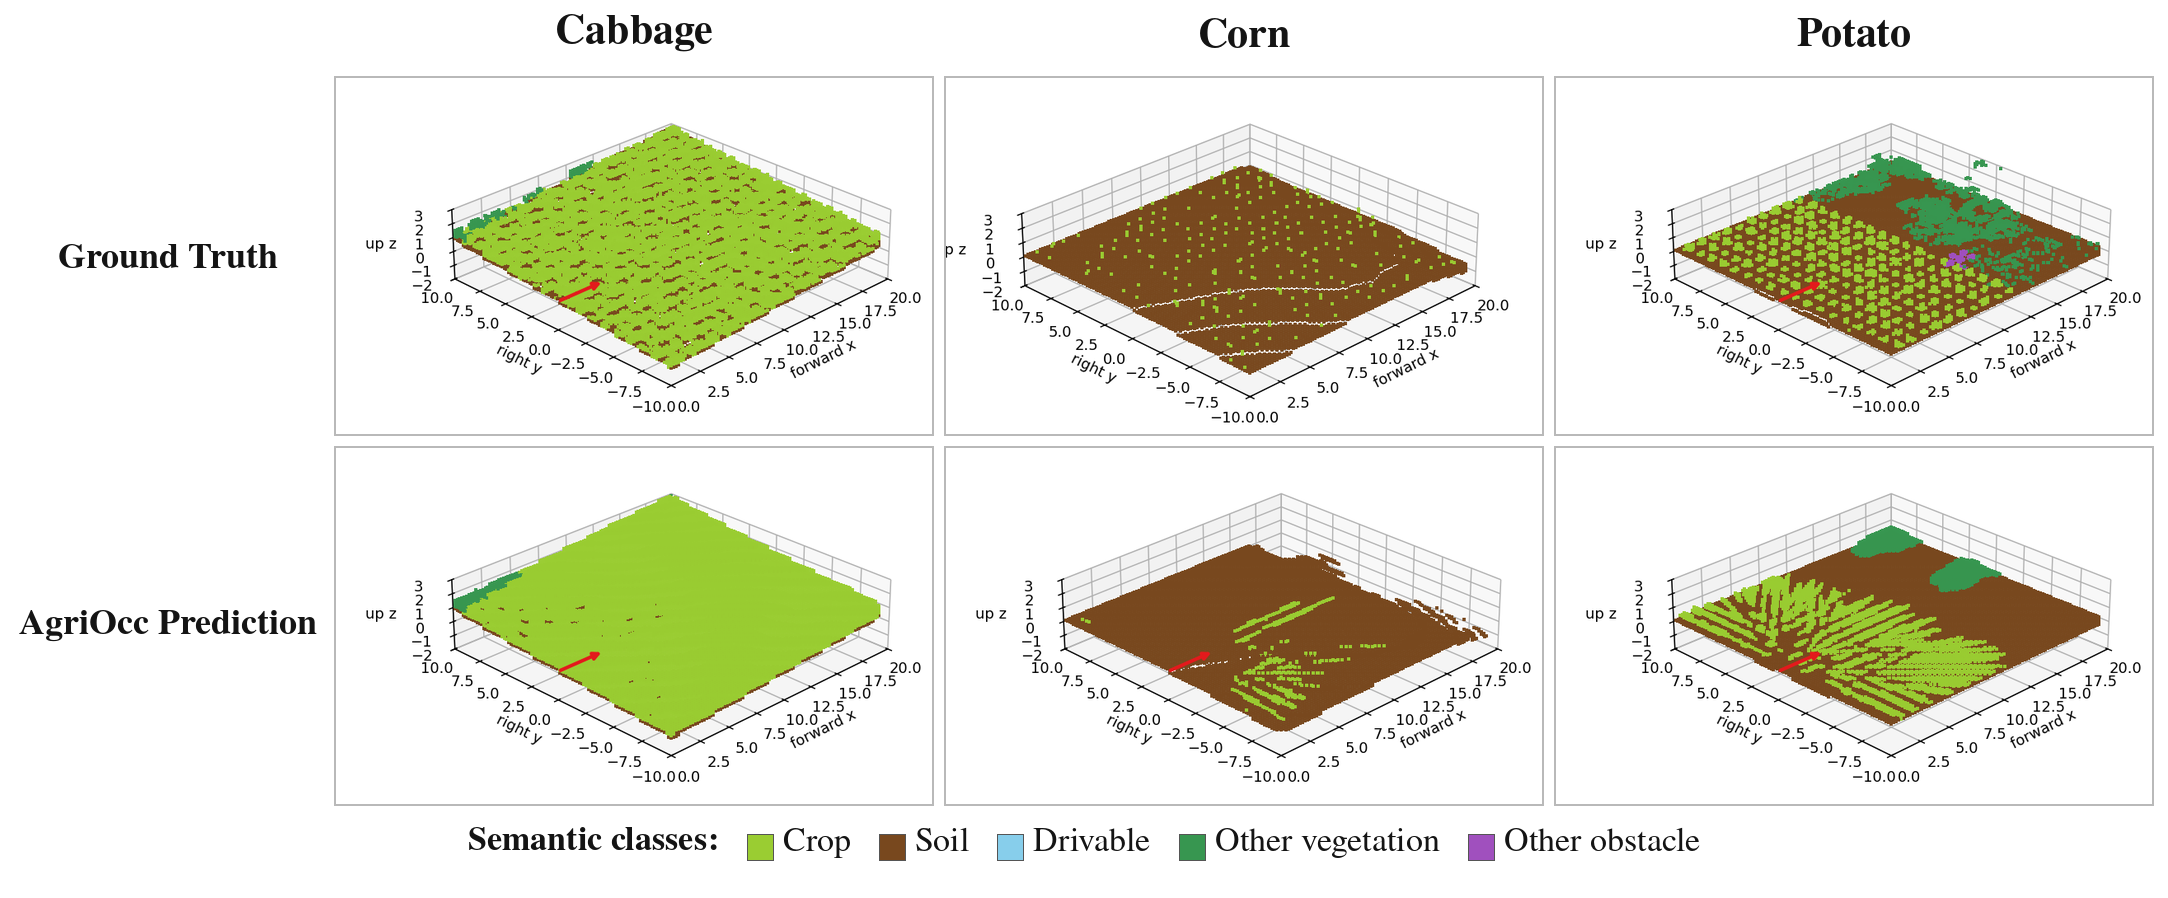
\includegraphics[width=\linewidth]{farmsim_limitations_2x3.png}
\caption{Examples of limitations on AgriOcc-Dataset. The first row shows ground truth and the second row shows AgriOcc predictions; columns show cabbage, corn, and potato scenes. Inter-plant gaps in dense crops tend to become connected regions, while small early-stage crops may be missed or incompletely recovered.}
\label{fig:limitations}\end{figure}

\section{Conclusion and future work}\label{sec:conclusion}
We proposed AgriOcc, which directly predicts current 3D semantic occupancy ahead of an agricultural robot in its coordinate frame from three forward-facing images. Its core components are the GeoVis-BEV encoder and the Agri-AMoE 3D occupancy decoder. GeoVis-BEV constructs anchor context from reliably visible regions with GVAD while preserving local deformable sampling, and the NearFar query layout prioritizes encoding budget for fine near-field structures. Agri-AMoE lifts final BEV representations to a 3D mixture-of-experts volume adaptively routed by gradient energy. AgriOcc achieves 56.99\% mIoU with 55.74M parameters on AgriOcc-Dataset; ORAD-3D results show that AgriOcc-Dataset pretraining provides an effective initialization for real off-road and farmland occupancy.

AgriOcc encodes crops, ground, free space, and obstacles as a unified 3D semantic interface directly usable for planning. GeoVis-BEV supplies geometry-aware representations for agricultural forward views, while Agri-AMoE turns them into 3D occupancy features suitable for multiple spatial structures. The paradigm can support dynamic operational-scene modeling, finer inter-plant-gap and plant-structure representation, and semantic-occupancy-based traversability prediction, obstacle avoidance, and closed-loop planning.

Future work will develop richer cross-domain training strategies for real farmland illumination, weather, crop growth stages, and sensor perturbations; use selectively activated high-resolution near-field queries to improve plant-level gaps and fine boundaries; and tightly couple AgriOcc with risk-aware traversability analysis, trajectory optimization, and closed-loop navigation. Semantic occupancy may ultimately provide a stable 3D foundation-model interface connecting perception, decision making, and control in agricultural robots.

\section*{Data and code availability}
The construction process, class definitions, and label generation procedure for AgriOcc-Dataset are described in Section~\ref{sec:dataset_construction}. The dataset and code used in this study are planned for public release for non-commercial research upon paper acceptance.

\section*{Declaration of competing interest}
The authors declare that they have no known competing financial interests or personal relationships that could have appeared to influence the work reported in this paper.

\bibliographystyle{cas-model2-names}
\bibliography{references}
\end{document}
